\documentclass[11pt,a4paper]{article}

% --- Packages ---
\usepackage[utf8]{inputenc}
\usepackage[T1]{fontenc}
\usepackage{lmodern}
\usepackage[margin=1in]{geometry}
\usepackage{graphicx}
\usepackage{booktabs}
\usepackage{array}
\usepackage{xcolor}
\usepackage{enumitem}
\usepackage{titlesec}
\usepackage{fancyhdr}
\usepackage[hidelinks]{hyperref}
\usepackage{abstract}

% --- Colours ---
\definecolor{accent}{HTML}{2F6F8F}
\definecolor{warn}{HTML}{B23A2E}

% --- Headings ---
\titleformat{\section}{\large\bfseries\color{accent}}{\thesection}{0.6em}{}
\titleformat{\subsection}{\normalsize\bfseries}{\thesubsection}{0.6em}{}

% --- Header / footer ---
\pagestyle{fancy}
\fancyhf{}
\rhead{\small Supportive Emotion \& Distress Text Classifier}
\lhead{\small Project Report}
\cfoot{\thepage}
\renewcommand{\headrulewidth}{0.4pt}

% --- A reusable safety/disclaimer box ---
\newcommand{\disclaimerbox}[1]{%
  \begin{center}
  \fcolorbox{warn}{warn!6}{%
    \parbox{0.95\linewidth}{\small\color{warn!80!black}\textbf{$\triangle$\ Safety \&
    scope:} #1}}
  \end{center}}

\title{\vspace{-1.5em}\textbf{\color{accent}Supportive Emotion \& Distress\\ Text
Classifier}\\[0.3em]\large A Non-Clinical NLP System for Emotional-Tone Reflection}
\author{Naman \\ \small Data Analyst (Portfolio Project)}
\date{June 2026}

\begin{document}
\maketitle
\thispagestyle{fancy}

\disclaimerbox{This system classifies the \emph{tone} of written text. It does
\textbf{not} diagnose mental-health conditions and is not a substitute for
professional help. When urgent-distress language is detected it surfaces real
crisis resources rather than attempting to handle the situation itself.}

\begin{abstract}
\noindent This project builds an end-to-end Natural Language Processing (NLP)
system that classifies short text messages into six emotional tones --- neutral,
stress, anxiety, sadness, anger, and loneliness --- and, through a separate
rule-based safety layer, flags urgent-distress language. The system is built with
a TF--IDF feature representation and a Logistic Regression classifier, achieving a
\textbf{held-out macro-F1 of 0.866}. Crucially, the emotion classifier and the
distress detector are kept architecturally separate so that the high-recall safety
behaviour is never traded away for accuracy on ordinary tones. The report
documents the data pipeline, modelling choices, evaluation, ethical boundaries,
and limitations, and outlines a roadmap for future improvement.
\end{abstract}

% =====================================================================
\section{Executive Summary}
% =====================================================================
\textbf{Problem.} Students and young adults increasingly journal and reflect on
their feelings in writing, but have few lightweight tools to recognise emotional
patterns in that writing. The goal here is a \emph{reflection aid}: a tool that
reads the tone of a short message, responds supportively, and --- if the language
suggests a crisis --- points the user to real help.

\medskip
\noindent\textbf{Approach.} The system combines two independent components:
\begin{enumerate}[leftmargin=1.4em,itemsep=2pt]
  \item An \textbf{emotion-tone classifier} (TF--IDF $+$ Logistic Regression) that
        returns a tone and a confidence score.
  \item A \textbf{rule-based distress safety layer} that runs on the raw text,
        tuned for recall, and overrides everything else when it fires.
\end{enumerate}

\medskip
\noindent\textbf{Key results.}
\begin{itemize}[leftmargin=1.4em,itemsep=2pt]
  \item Held-out macro-F1: \textbf{0.866}; accuracy: \textbf{0.91} (2{,}000 unseen
        test messages).
  \item Distress safety layer: \textbf{100\% recall} on a labelled probe set
        (0 false negatives).
  \item Logistic Regression chosen over a marginally more accurate SVM because the
        product requires calibrated probabilities.
\end{itemize}

\medskip
\noindent\textbf{Headline judgement.} The most important design decision in this
project is \emph{not} a modelling one --- it is the choice to treat urgent distress
as a separate, auditable safety net rather than as another machine-learned class.
This protects the one outcome where errors carry real human cost.

% =====================================================================
\section{Data}
% =====================================================================
The model is trained on the public \texttt{dair-ai/emotion} dataset (English,
social-media text). Its six native labels are remapped onto the project's six
tones, and the two tones the source lacks are derived from curated keywords:

\begin{center}
\begin{tabular}{@{}ll@{}}
\toprule
\textbf{Source label} & \textbf{Mapped tone} \\
\midrule
sadness & sadness \\
anger & anger \\
fear & anxiety \\
joy / love / surprise & neutral \\
\midrule
(keyword-derived from sadness) & loneliness \\
(keyword-derived from anxiety/neutral) & stress \\
\bottomrule
\end{tabular}
\end{center}

\noindent After remapping and capping at 2{,}500 samples per class to reduce
imbalance, the training set contains \textbf{9{,}432 rows}. Evaluation uses the
dataset's own held-out test split (2{,}000 rows) --- data never seen in training.

\disclaimerbox{The \texttt{stress} and \texttt{loneliness} classes are
\emph{keyword-derived} because the source dataset has no native label for them.
They are therefore noisier and data-starved; this is a known limitation, not a
defect, and is the top data-collection priority for any future version.}

% =====================================================================
\section{Methodology}
% =====================================================================
\subsection{Preprocessing}
Text is lower-cased, stripped of URLs and \texttt{@}-mentions (which also
anonymises handles), and lemmatised. Two deliberate choices matter:
\begin{itemize}[leftmargin=1.4em,itemsep=2pt]
  \item \textbf{Negations are kept} (\emph{not, no, never}). Removing them with a
        generic stop-word list would turn ``not okay'' into ``okay'' and silently
        invert meaning --- the single most important preprocessing decision.
  \item \textbf{Intensity punctuation (\texttt{!\,?}) is retained}, since it carries
        emotional signal.
\end{itemize}

\subsection{Features and Model}
Cleaned text is vectorised with TF--IDF over unigrams and bigrams
(\texttt{ngram\_range=(1,2)}), capturing phrases such as ``not okay'' as single
features. A Logistic Regression classifier with \texttt{class\_weight="balanced"}
is trained on top. TF--IDF up-weights distinctive words and down-weights common
ones; Logistic Regression is fast, interpretable, and --- importantly for this
product --- exposes per-class probabilities.

\subsection{The Distress Safety Layer}
The distress detector is an auditable set of regular expressions run on the
\emph{raw} text (before any cleaning could strip critical words). It is
intentionally \emph{not} a machine-learned model: where a false negative carries
serious cost, a transparent rule set tuned for recall is the responsible choice.
Its output is a separate field that is never folded into, or overwritten by, the
emotion prediction.

% =====================================================================
\section{Results}
% =====================================================================
\subsection{Model Comparison (5-fold CV macro-F1)}
\begin{center}
\begin{tabular}{@{}lcl@{}}
\toprule
\textbf{Model} & \textbf{macro-F1} & \textbf{Note} \\
\midrule
Linear SVM & 0.902 & highest, but no \texttt{predict\_proba} \\
\textbf{Logistic Regression} & \textbf{0.879} & \textbf{chosen} --- gives confidence scores \\
Naive Bayes & 0.588 & weak baseline \\
\bottomrule
\end{tabular}
\end{center}

\noindent We ship Logistic Regression rather than the SVM: the product needs
per-class probabilities (a confidence score and a probability bar chart), and a
$\sim$2-point F1 gap does not justify losing them.

\subsection{Per-Class Performance (held-out test)}
\begin{center}
\begin{tabular}{@{}lcccc@{}}
\toprule
\textbf{Tone} & \textbf{Precision} & \textbf{Recall} & \textbf{F1} & \textbf{Support} \\
\midrule
anger      & 0.85 & 0.88 & 0.87 & 275 \\
anxiety    & 0.83 & 0.90 & 0.86 & 202 \\
loneliness & 0.79 & 0.90 & 0.84 & 30 \\
neutral    & 0.95 & 0.93 & 0.94 & 907 \\
sadness    & 0.93 & 0.89 & 0.91 & 551 \\
stress     & 0.69 & 0.89 & 0.78 & 35 \\
\midrule
\textbf{macro avg} & 0.84 & 0.90 & \textbf{0.87} & 2{,}000 \\
\bottomrule
\end{tabular}
\end{center}

\subsection{Confusion Matrix}
Figure~\ref{fig:cm} shows the held-out confusion matrix. The diagonal dominates,
and the off-diagonal errors are \emph{sensible} rather than random: sadness blurs
into neutral and anger, and mildly negative ``neutral'' text drifts toward
anxiety or sadness. The keyword-derived classes (loneliness, stress) separate
surprisingly cleanly, though their small support means these figures should be
read with caution.

\begin{figure}[h]
  \centering
  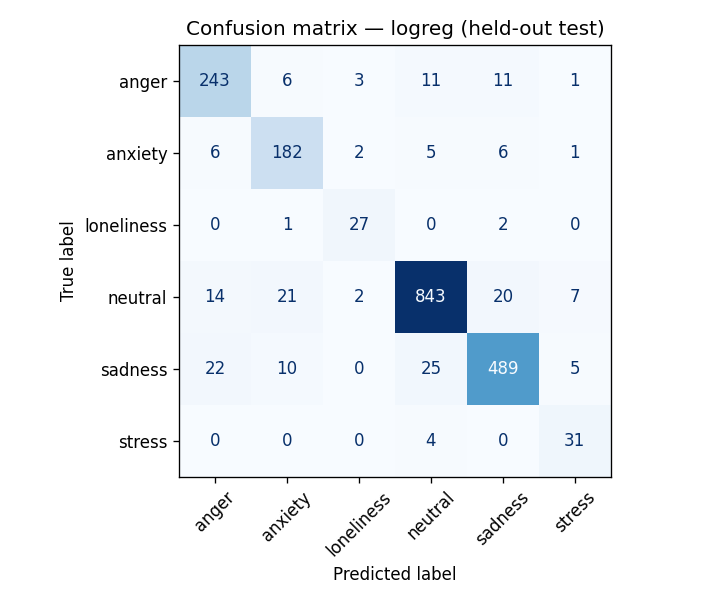
\includegraphics[width=0.72\linewidth]{confusion_matrix.png}
  \caption{Held-out confusion matrix (Logistic Regression). Rows are the true
  tone; columns are the predicted tone.}
  \label{fig:cm}
\end{figure}

\subsection{Distress Safety Layer}
On a labelled probe set the layer achieved \textbf{100\% recall} (5/5 true-distress
messages caught, 0 false negatives, 0 false alarms). This metric is reported
separately and deliberately prioritises recall: a missed true-distress message is
the costliest error in the system, and false positives are an acceptable price.

% =====================================================================
\section{Ethical Considerations}
% =====================================================================
\begin{itemize}[leftmargin=1.4em,itemsep=2pt]
  \item \textbf{Tone, not diagnosis.} The tool describes the tone of words
        (``this sounds anxious''), never a person's condition (``you have
        anxiety'').
  \item \textbf{Separation of safety.} Distress detection is decoupled from the
        emotion model so safety behaviour cannot be diluted by accuracy
        optimisation.
  \item \textbf{Privacy.} Only derived signals (tone, confidence, distress flag,
        timestamp) are logged --- never the user's raw text.
  \item \textbf{Crisis hand-off.} When distress is detected, the system shows
        verified crisis resources rather than attempting to respond itself.
\end{itemize}

% =====================================================================
\section{Limitations}
% =====================================================================
\begin{itemize}[leftmargin=1.4em,itemsep=2pt]
  \item \texttt{joy}/\texttt{love}/\texttt{surprise} are collapsed into
        \texttt{neutral}; here ``neutral'' means ``not a negative tone''.
  \item \texttt{stress} and \texttt{loneliness} are keyword-derived, noisier, and
        data-starved (n$=$35 and n$=$30 in test).
  \item Trained on English social-media text only $\rightarrow$ register and
        demographic bias.
  \item TF--IDF matches words, not meaning: sarcasm and context are not
        understood.
  \item The distress layer will miss indirect or coded language --- it is a safety
        net, not a guarantee.
\end{itemize}

% =====================================================================
\section{Future Work}
% =====================================================================
\begin{enumerate}[leftmargin=1.4em,itemsep=2pt]
  \item Collect real labelled \texttt{stress} and \texttt{loneliness} examples to
        replace keyword derivation.
  \item Replace TF--IDF with Sentence-Transformer embeddings (e.g.
        \texttt{all-MiniLM-L6-v2}) and measure the lift.
  \item Add SHAP/LIME explanations for per-prediction transparency.
  \item Calibrate probabilities so confidence scores are trustworthy.
  \item Localise crisis resources and add multilingual support.
\end{enumerate}

\vspace{1em}
\disclaimerbox{This is a reflection aid for educational and portfolio purposes ---
\textbf{not} a clinical or crisis tool. Crisis resources referenced by the system
must be verified and localised before any real-world use.}

\end{document}
